% Source: graduate-coursework/Prior_Semesters/Sp24/EMCH354/assignments/HW2/HW2.tex

\documentclass[border=4pt]{standalone}
\usepackage{amsmath}
\usepackage{tikz}
\usetikzlibrary{patterns}
\usetikzlibrary{arrows.meta, decorations.pathmorphing}

\definecolor{bluecolor}{RGB}{173,216,230}
\definecolor{purplecolor}{RGB}{210,180,222}
\definecolor{pinkcolor}{RGB}{255,182,193}
\definecolor{orangecolor}{RGB}{252, 213, 180}

\begin{document}
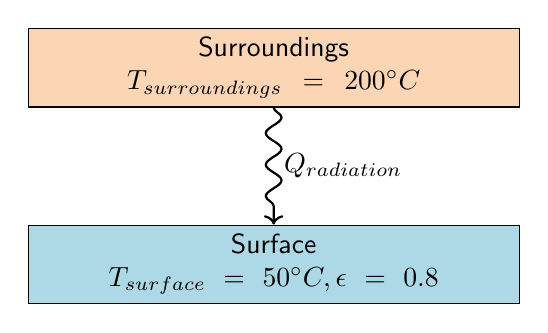
\begin{tikzpicture}[font=\sffamily]
    % Define the style for the surfaces
    \tikzstyle{surface} = [draw, fill=bluecolor, text width=6cm, minimum height=1cm, align=center]

    % Surface with lower temperature (receiving heat)
    \node[surface] (surface) at (0,0) {Surface \\ \( T_{surface} = 50^\circ C, \epsilon = 0.8 \)};

    % Surroundings with higher temperature (emitting heat)
    \node[surface, fill=orangecolor] (surroundings) at (0,2.5) {Surroundings \\ \( T_{surroundings} = 200^\circ C \)};

    % Radiation heat transfer arrows (pointing from the surroundings to the surface)
    \draw[->,thick, decorate, decoration={snake, amplitude=1mm, segment length=4mm, post length=1mm}] (surroundings.south) -- (surface.north)
        node[midway,right] {\( Q_{radiation} \)};
\end{tikzpicture}
\end{document}
